% flashcards-title: Three same-size wholes each cut into four equal pieces
% flashcards-desc: Three identical rectangles side by side, each divided by vertical lines into four equal pieces. The first piece of the first rectangle is labeled one fourth in fraction notation.
\documentclass[tikz]{standalone}
\usetikzlibrary{arrows.meta,patterns}

\definecolor{qraNavy}{HTML}{17324D}
\definecolor{qraBlue}{HTML}{2B6CB0}
\definecolor{qraGold}{HTML}{B7791F}
\definecolor{qraPale}{HTML}{EAF2F8}
\definecolor{qraGray}{HTML}{5C6773}

\tikzset{
  qra axis/.style={draw=qraNavy, line width=1.2pt},
  qra tick/.style={draw=qraNavy, line width=1pt},
  qra guide/.style={draw=qraGray, densely dashed, line width=0.8pt},
  qra counter/.style={circle, draw=qraNavy, fill=qraPale, line width=0.9pt, minimum size=7mm, inner sep=0pt},
  qra label/.style={font=\sffamily\bfseries, text=qraNavy},
  qra small label/.style={font=\sffamily, text=qraNavy},
}

\begin{document}
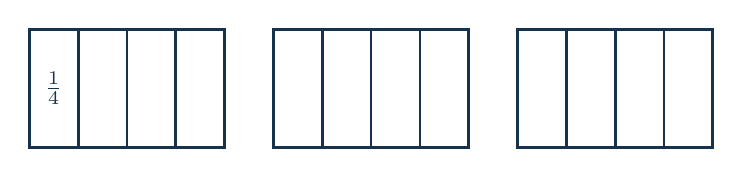
\begin{tikzpicture}[x=0.62cm, y=1.5cm]
  \foreach \w in {0,1,2} {
    \begin{scope}[shift={({\w*5},0)}]
      \foreach \i in {1,...,3} \draw[qra tick] (\i,0) -- (\i,1);
      \draw[qra axis] (0,0) rectangle (4,1);
    \end{scope}
  }
  \node[qra small label] at (0.5,0.5) {$\frac{1}{4}$};
\end{tikzpicture}
\end{document}
